\documentclass[a4paper,oneside,12pt]{book}
\usepackage{BUPTthesisbachelor}
\usepackage{setspace}

\usepackage[final]{pdfpages}

\usepackage{listings}
\usepackage{xcolor}

\usepackage{amssymb}
\usepackage{bm}

\usepackage{algorithm}  
\usepackage{algorithmicx}  
\usepackage{algpseudocode}  

\lstdefinestyle{sharpc}{language=[Sharp]C, frame=lrtb, rulecolor=\color{blue!80!black}}


%%%%%%%%%%%%%%%%%%%%%%%%% Begin Documents %%%%%%%%%%%%%%%%%%%%%%%%%%
\begin{document}

% 封面

\includepdf[pages=-]{docs/cover.pdf}  
\newpage

% 任务书
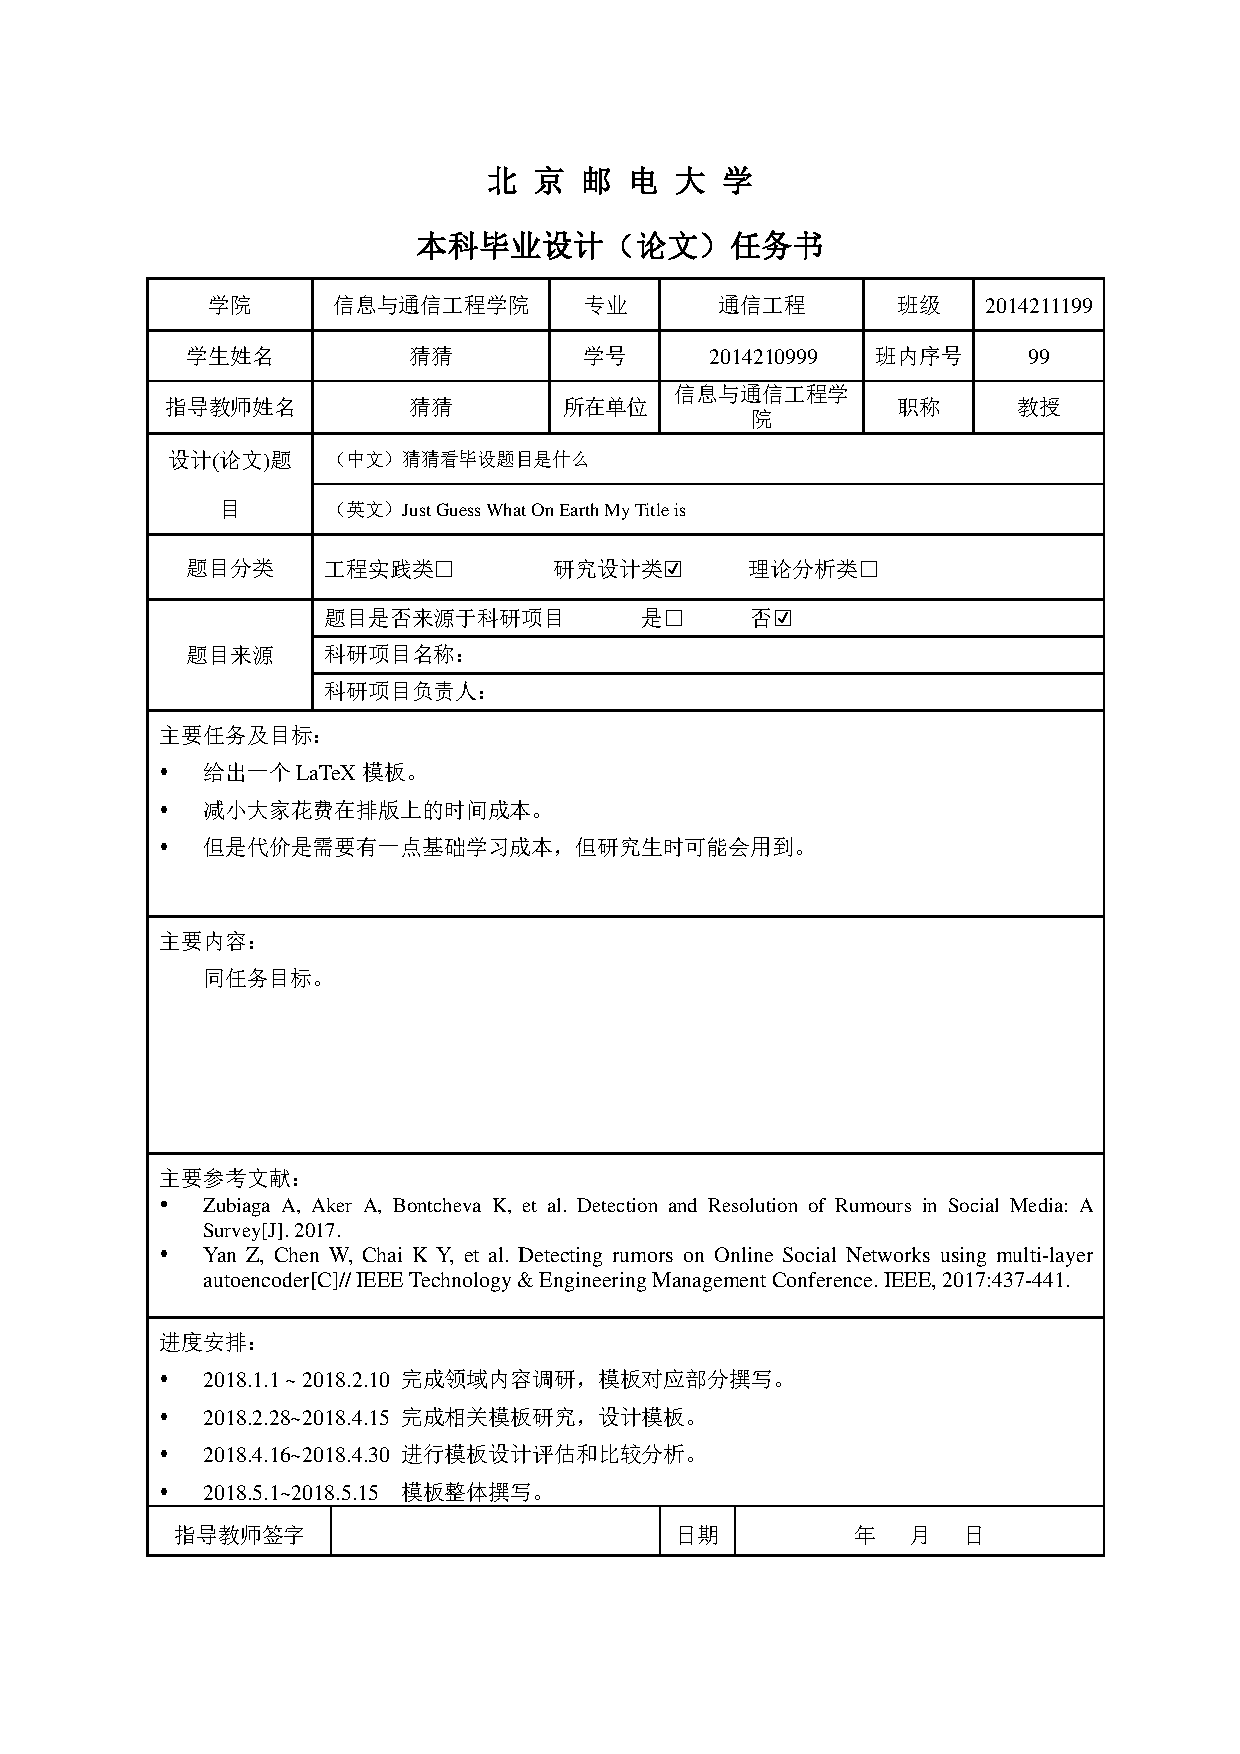
\includepdf[pages=-]{docs/task.pdf}  
\newpage

% 成绩评定表
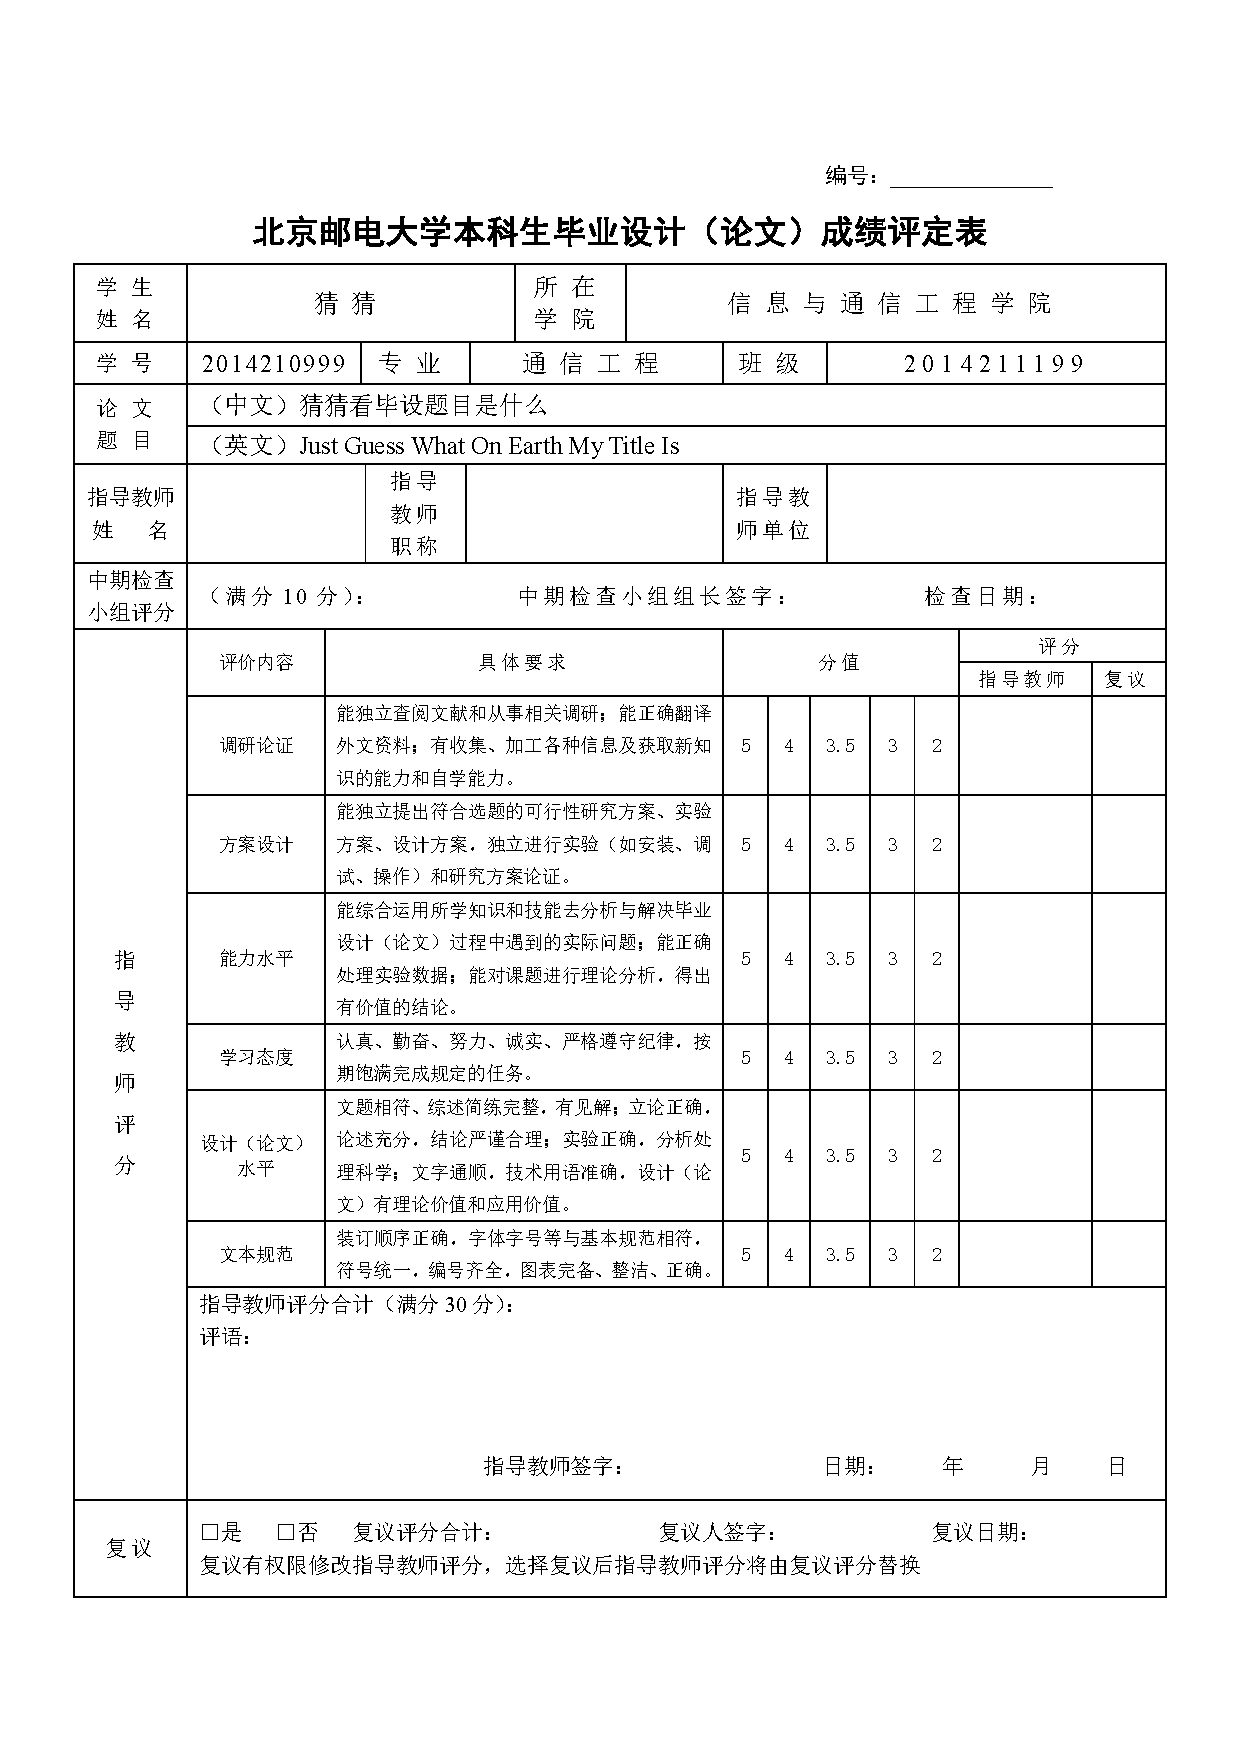
\includepdf[pages=-]{docs/scoreTable.pdf}  
\newpage

% 诚信声明

\includepdf[pages=-]{docs/statement.pdf} 
\newpage

%%%%%%%%%%%%%%%%%%%%%%%%%%%%%%%%%%%%%%%%%%%%%%%%%%%%%%%%%%%%%%%%%%%%
%                                                                  %
%   Copyright (c) 2010 - 2011 Caspar Zhang <casparant@gmail.com>   %
%                                                                  %
%   This copyrighted material is made available to anyone wishing  %
%   to use, modify, copy, or redistribute it subject to the terms  %
%   and conditions of the GNU General Public License version 2.    %
%                                                                  %
%   This program is distributed in the hope that it will be        %
%   useful, but WITHOUT ANY WARRANTY; without even the implied     %
%   warranty of MERCHANTABILITY or FITNESS FOR A PARTICULAR        %
%   PURPOSE. See the GNU General Public License for more details.  %
%                                                                  %
%   You should have received a copy of the GNU General Public      %
%   License along with this program; if not, write to the Free     %
%   Software Foundation, Inc., 51 Franklin Street, Fifth Floor,    %
%   Boston, MA 02110-1301, USA.                                    %
%                                                                  %
%%%%%%%%%%%%%%%%%%%%%%%%%%%%%%%%%%%%%%%%%%%%%%%%%%%%%%%%%%%%%%%%%%%%

% 你只需要修改下面几行就可以完成大部分内容的填写,
% 这要求你具有一定的LaTeX基础,但是如果你足够聪明,
% 不具有LaTeX基础也可以完成。

% 论文中文题目
\def\thesistitle{社猜猜看这个毕设题目是什么}

% 论文英文题目
%提示:英文摘要页的标题注意格式要求。
\def\thesistitleen{HAVE A TRY TO GUESS WHAT THE TITLE IS}

% Thank Words
\def\thankwords{

此处请写致谢的内容。

它可以有多段。
}
    % Main items 
%%%%%%%%%%%%%%%%%%%%%%%%%%%%%%%%%%%%%%%%%%%%%%%%%%%%%%%%%%%%%%%%%%%%
%                                                                  %
%   Copyright (c) 2010 - 2011 Caspar Zhang <casparant@gmail.com>   %
%                                                                  %
%   This copyrighted material is made available to anyone wishing  %
%   to use, modify, copy, or redistribute it subject to the terms  %
%   and conditions of the GNU General Public License version 2.    %
%                                                                  %
%   This program is distributed in the hope that it will be        %
%   useful, but WITHOUT ANY WARRANTY; without even the implied     %
%   warranty of MERCHANTABILITY or FITNESS FOR A PARTICULAR        %
%   PURPOSE. See the GNU General Public License for more details.  %
%                                                                  %
%   You should have received a copy of the GNU General Public      %
%   License along with this program; if not, write to the Free     %
%   Software Foundation, Inc., 51 Franklin Street, Fifth Floor,    %
%   Boston, MA 02110-1301, USA.                                    %
%                                                                  %
%%%%%%%%%%%%%%%%%%%%%%%%%%%%%%%%%%%%%%%%%%%%%%%%%%%%%%%%%%%%%%%%%%%%

% 你只需要修改下面内容就可以完成中英文摘要,
% 这要求你具有一定的LaTeX基础,但是还是那句话,
% 如果你足够聪明,不具有LaTeX基础也可以完成。

% 中文摘要
\def\abstractcn{
%从这里开始写你的摘要,分段需要空一行。
这是中文摘要的部分。

它可以拥有多段。
这是中文摘要的部分。

它可以拥有多段。

如果你写的太长,甚至可以到第二页。
%摘要结束
}

% 中文关键字 
% TODO: 改成可变长度的
\def\abscnkeyone{北京邮电大学}
\def\abscnkeytwo{本科生}
\def\abscnkeythree{毕业设计}
\def\abscnkeyfour{模板}
\def\abscnkeyfive{示例}

% ABSTRACT
\def\abstracten{
%Your abstract here, to make a new paragraph, give an extra blank line please.
This is ABSTRACT.

You can write more than one paragraph here.

If your abstract is too long, it will take up more pages. 
%Abstract done
}

% Key Words 
% TODO: 改成可变长度的
\def\absenkeyone{BUPT}
\def\absenkeytwo{undergraduate}
\def\absenkeythree{thesis}
\def\absenkeyfour{template}
\def\absenkeyfive{example}


  % Abstract
\frontmatter\tableofcontents % Content

% 正文
\newpage\mainmatter
\fancypagestyle{plain}{\pagestyle{fancy}} % Add head to new chapter
\pagestyle{fancy} % Head and foot
%\let\cleardoublepagebak=\cleardoublepage
%\let\cleardoublepage\relax % Make new chapter stay on old page

%%%%%%%%%%%%%%%%%%%%%%%%%%%%% Main Area %%%%%%%%%%%%%%%%%%%%%%%%%%%%

\chapter{基础模块示例}
\section{特殊文本类型}
\subsection{脚注}
社交媒体是一种供用户创建在线社群来分享信息、观点、个人信息和其它内容(如视频)的电子化交流平台,社交网络服务(social network service, SNS)和微博客(microblogging)都属于社交媒体的范畴\cite{webster_social_media},国外较为知名的有Facebook\footnote{http://www.facebook.com/}、Instagram\footnote{https://www.instagram.com/}、Twitter\footnote{http://www.twitter.com/}、LinkedIn\footnote{http://www.linkedin.com/}等,国内较为知名的有新浪微博\footnote{http://www.weibo.com/}。

在社交媒体的强覆盖下,新闻信息的传播渠道也悄然了发生变化。

\subsection{定义}
\begin{definition}
社交媒体新闻是指社交媒体平台的用户通过网络自发进行创作,并在平台上进行共享传播的文字、语音、视频等信息,是用户生成内容(UGC)的一种。\cite{周兴2017基于深度学习的谣言检测及模式挖掘}
\end{definition}

\subsection{中英文文献、学位论文引用}
根据美国皮尤研究中心的2017年9月发布的调查结果\cite{pew_news_use_2017},67\%的美国民众会从社交媒体上获取新闻信息,其中高使用频率用户占20\%。在国内,中国互联网信息中心《2016年中国互联网新闻市场研究报告》\cite{internet_news_2016}也显示,社交媒体已逐渐成为新闻获取、评论、转发、跳转的重要渠道,在2016年下半年,曾经通过社交媒体获取过新闻资讯的用户比例高达90.7\%,在微信、微博等社交媒体参与新闻评论的比例分别为62.8\%和50.2\%。社交媒体正在成为网络上热门事件生成并发酵的源头,在形成传播影响力后带动传统媒体跟进报道,最终形成更大规模的舆论浪潮。

在国内,新浪微博由于其发布方便、传播迅速、受众广泛且总量大的特点,成为了虚假信息传播的重灾区:《中国新媒体发展报告(2013)》\cite{唐绪军2013中国新媒体发展报告}显示,2012年的100件微博热点舆情案例中,有超过1/3出现谣言;《中国新媒体发展报告(2015)》\cite{唐绪军2015中国新媒体发展报告}对2014年传播较广、比较典型的92条假新闻进行了多维度分析,发现有59\%的虚假新闻首发于新浪微博。

此等信息的传播严重损害了有关公众人物的名誉权,降低了社交媒体服务商的商业美誉度,扰乱了网络空间秩序,冲击着网民的认知,极易对民众造成误导,带来诸多麻烦和经济损失,甚至会导致社会秩序的混乱。针对社交媒体谣言采取行动成为了有关部门、服务提供商和广大民众的共同选择。\cite{周兴2017基于深度学习的谣言检测及模式挖掘}

\section{图表及其引用}
此处引用了表\ref{crowdwisdom}。

\begin{bupttable}{基于浏览者行为的特征}{crowdwisdom}
    \begin{tabular}{l|l|l}
		\hline \textbf{特征} & \textbf{描述} & \textbf{形式与理论范围}\\
		\hline 点赞量 & 微博的点赞数量 & 数值,$\mathbb{N}$ \\
		\hline 评论量 & 微博的评论数量 & 数值,$\mathbb{N}$ \\
		\hline 转发量 & 微博的转发数量 & 数值,$\mathbb{N}$ \\
		\hline
    \end{tabular}
\end{bupttable}

此处引用了一张图。图\ref{autoencoder}表示的是一个由含有4个神经元的输入层、含有3个神经元的隐藏层和含有4个神经元的输出层组成的自编码器,$+1$代表偏置项。

\buptfigure{pictures/autoencoder}{自编码器结构}{autoencoder}


\section{公式与算法表示}

\subsection{例子:基于主成分分析}
下面对主成分分析进行介绍。

主成分分析是一种简单的机器学习算法,其功能可以从两方面解释:一方面可以认为它提供了一种压缩数据的方式,另一方面也可以认为它是一种学习数据表示的无监督学习算法。\cite{Goodfellow2016DeepLearning}
通过PCA,我们可以得到一个恰当的超平面及一个投影矩阵,通过投影矩阵,样本点将被投影在这一超平面上,且满足最大可分性(投影后样本点的方差最大化),直观上讲,也就是能尽可能分开。

对中心化后的样本点集$\bm{X}=\{\bm{x}_1,\bm{x}_2,\ldots,\bm{x}_i,\ldots,\bm{x}_m\}$(有$\sum_{i=1}^{m}\bm{x}_i = 0$),考虑将其最大可分地投影到新坐标系\ $\bm{W}= \{\bm{w}_1,\bm{w}_2,\ldots,\bm{w}_i,\ldots,\bm{w}_d\} $,其中$\bm{w}_i$是标准正交基向量,满足$\|\bm{w}_i\|_2 = 1$, $\bm{w}_i^T\bm{w}_j = 0$($i \not= j$)。假设我们需要$d^\prime$($d^\prime < d$)个主成分,那么样本点$\bm{x}_i$在低维坐标系中的投影是$\bm{z}_i = (z_{i1};z_{i2};\ldots;z_{id^\prime})$,其中$z_{ij} = \bm{w}_j^\mathrm{T}\bm{x}_i$,是$\bm{x}_i$在低维坐标系下第$j$维的坐标。
对整个样本集,投影后样本点的方差是
\begin{equation}
\begin{aligned}
    & \frac{1}{m}\sum_{i=1}^m \bm{z}_i^\mathrm{T}\bm{z}_i \\
= & \frac{1}{m}\sum_{i=1}^m (\bm{x}_i^\mathrm{T}\bm{W})^\mathrm{T}(\bm{x}_i^\mathrm{T}\bm{W}) \\
= & \frac{1}{m}\sum_{i=1}^m \bm{W}^\mathrm{T}\bm{x}_i\bm{x}_i^\mathrm{T}\bm{W} \\
= & \frac{1}{m} \bm{W}^\mathrm{T}\bm{X}\bm{X}^\mathrm{T}\bm{W} \\
\end{aligned}
\end{equation}

由于我们知道新坐标系$\bm{W}$的列向量是标准正交基向量,且样本点集$\bm{X}$已经过中心化,则PCA的优化目标可以写为
\begin{equation}
\label{PCA_goal}
\begin{aligned}
& \max_{\substack{\bm{W}}}  &  tr(\bm{W}^\mathrm{T}\bm{X}\bm{X}^ \mathrm{T}\bm{W}) \\
& \operatorname{ s.t. }  &  \bm{W}^\mathrm{T}\bm{W} = \bm{I} \\
\end{aligned}
\end{equation}

由于$\bm{X}\bm{X}^ \mathrm{ T }$是协方差矩阵,那么只需对它做特征值分解,即
\begin{equation}
\label{PCA_eigenvalue}
\bm{X}^ \mathrm{ T }\bm{X} = \bm{W}\bm{\Lambda}\bm{W}^ \mathrm{ T } \\
\end{equation}
其中$\bm{\Lambda}=diag(\bm{\lambda})$,$\bm{\lambda} = \{\lambda_1,\lambda_2,\ldots,\lambda_m\}$。

具体地,考虑到它是半正定矩阵的二次型,存在最大值,可对\eqref{PCA_goal}使用拉格朗日乘数法
\begin{equation}
\bm{X}\bm{X}^ \mathrm{ T }\bm{w}_i  = \lambda_i \bm{w}_i \\
\end{equation}

之后将求得的特征值降序排列,取前$d^\prime$个特征值对应的特征向量组成所需的投影矩阵$\bm{W}^\prime =(\bm{w}_1,\bm{w}_2,\ldots,\bm{w}_{d^\prime})$,即可得到PCA的解。PCA算法的描述如算法\ref{PCA_algorithm}所示。
\begin{algorithm} 
\floatname{algorithm}{算法}
\caption{主成分分析(PCA)} 
\label{PCA_algorithm}
\renewcommand{\algorithmicrequire}{\textbf{输入:}}
\renewcommand{\algorithmicensure}{\textbf{输出:}} 
\begin{algorithmic}[1] 
\Require 样本集$\bm{x}=\{\bm{x}_1,\bm{x}_2,\ldots,\bm{x}_i,\ldots,\bm{x}_m\}$,低维空间维数$d^\prime$ 
\Ensure 投影矩阵  $\bm{W}^\prime =(\bm{w}_1,\bm{w}_2,\ldots,\bm{w}_{d^\prime})$
\State 对所有样本中心化$\bm{x}_i \gets \bm{x}_i - \frac{1}{m}\sum_{i=1}^m \bm{x}_i$
\State  计算样本的协方差$\bm{X}\bm{X}^ \mathrm{T}$
\State 对协方差矩阵$\bm{X}\bm{X}^ \mathrm{T}$做特征值分解
\State 取最大的$d^\prime$个特征值所对应的特征向量$\bm{w}_1,\bm{w}_2,\ldots,\bm{w}_{d^\prime}$
\end{algorithmic}  
\end{algorithm}

论文\cite{Chen2016Behavior}认为,通过PCA保留一定的主成分,可以更好地把握历史微博的共性,使历史上的非谣言微博与谣言微博产生可度量的距离。

论文采取了排序的检测方式:如果待判别的微博在特征空间中距离非谣言微博数据的“重心”比任何非谣言微博都要远,即成为了离群点,则认为该微博是一条谣言。但考虑到实验过程中应尽量统一化比较手段,在本节中,我们采用了Yan Zhang论文\cite{Yan2017OneHot}中的阈值法来进行判别:在特征空间中,如果待判定微博没有阈值范围内的相邻点,则认为该微博是一条谣言。

记待判定微博$\bm{w}_0$的经典特征向量为$\bm{f}^{c}_{0}$,它的发布者在$\bm{w_0}$前发布的$k$条微博为$\bm{W} = \bm{w}_1,\bm{w}_2,\ldots,\bm{w}_k$,这$k$条微博对应的经典特征向量集为$\bm{F}^{c}_{W} = \{ \bm{f}^{c}_{1},\bm{f}^{c}_{2},\ldots,\bm{f}^{c}_{k} \}$。令$label = 1$代表谣言,$label = 0$代表非谣言。算法的具体流程如算法\ref{PCA_model}所示。

\begin{algorithm} 
\floatname{algorithm}{算法}
\caption{基于PCA的信息可信度评估} 
\label{PCA_model}
\renewcommand{\algorithmicrequire}{\textbf{输入:}}
\renewcommand{\algorithmicensure}{\textbf{输出:}} 
	\begin{algorithmic}[1] 
	\Require $\bm{f}^{c}_{0}$,$\bm{F}^{c}_{W}$,保留主成分数$n$
	\Ensure 标签$label\in \{0,1\}$
	\State 对所有特征向量应用PCA,保留前$n$个主成分$\bm{o}^{c}_{i} \gets PCA(\bm{f}^{c}_{i}, n)$($i = 0,1,\ldots,k$)
	\State 计算$\bm{F}^{c}_{W}$中各向量的平均距离$\mu$和标准差$\sigma$
	\State 计算阈值$thr = {\mu} / {\sigma}$
	\If {$\min_{1<j\le k} \|\bm{o}^{c}_{0} - \bm{o}^{c}_{j} \|_2 > thr$}
		\State $ label \gets 1 $
	\Else
		\State $ label \gets 0 $
	\EndIf
	\end{algorithmic}
\end{algorithm}

\section{代码表示}
下面的代码\ref{plus}是用Python编写的加法函数。

\begin{lstlisting}[language=Python, caption=加法, label=plus, tabsize=2]  
def plus_func(a,b):
	return a+b
\end{lstlisting}  

\section{列表样式}

以下是使用圆点作为项目符号的列表样式。

\begin{itemize}
\item \textbf{第一章为基础模块示例},是的,就是本章。
\item \textbf{第二章为不存在},是的,其实它不存在。
\end{itemize}

以下是使用数字作为项目符号的列表样式。

\begin{enumerate}
\item \textbf{第一章为基础模块示例},是的,就是本章。
\item \textbf{第二章为不存在},是的,其实它不存在。
\end{enumerate}

以下是无项目符号(实际是可以自定义一些符号,但我懒得加了)的列表样式,它会顶格书写。

\begin{description}
\item \textbf{第一章为基础模块示例},是的,就是本章。
\item \textbf{第二章为不存在},是的,其实它不存在。
\end{description}

%%%%%%%%%%%%%%%%%%%%%%% Main Area ENDs Here %%%%%%%%%%%%%%%%%%%%%%%%
%\let\cleardoublepage=\cleardoublepagebak
% Reference
\clearpage\phantomsection\addcontentsline{toc}{chapter}{参考文献}
\bibliographystyle{buptbachelor}
\refbodyfont{\bibliography{ref}}

% Thanks to page
\clearpage\phantomsection\addcontentsline{toc}{chapter}{致\qquad{}谢}
\chapter*{致\qquad{}谢}
\normalsize\thankwords

% Appendix
\chapter*{附\qquad{}录}
\phantomsection\addcontentsline{toc}{chapter}{附\qquad{}录}

\phantomsection
\addcontentsline{toc}{section}{附录1\quad{}缩略语表}
\section*{附录1\quad{}缩略语表}
\begin{center}
	\begin{tabular}{ccc}
		\textbf{英文缩写} & \textbf{英文名称} & \textbf{中文} \\
		\hline
		AE & autoencoder & 自编码器\\
		CRF & conditional random field & 条件随机场\\
		LR & logistic regression & 逻辑回归\\
		LSTM & Long Short Term Memory & 长短时记忆单元 \\
	\end{tabular}
\end{center}

\phantomsection
\addcontentsline{toc}{section}{附录2\quad{}数学符号}
\section*{附录2\quad{}数学符号}
\begin{center}
	\begin{tabular}{ccc}
		\multicolumn{2}{c}{\textbf{数和数组}} \\
		\\
		$a$ & 标量(整数或实数)\\
		$\bm{a}$ & 向量\\
		$dim()$ & 向量的维数\\
		$\bm{A}$ & 矩阵\\
		$\bm{A}^\mathrm{T}$ & 矩阵$\textbf{A}$的转置\\
		$\bm{I}$ & 单位矩阵(维度依据上下文而定) \\
 		$diag(\bm{a})$ & 对角方阵,其中对角元素由向量$\bm{a}$确定 \\

	\end{tabular}
\end{center}

\newpage\backmatter
% Translation
\chapter*{外\quad{}文\quad{}译\quad{}文}
\vspace{8mm}

\thispagestyle{empty}

\begin{center}
\sihao\heiti{真假新闻的在线传播}

\xiaosihao\songti{Soroush Vosoughi, Deb Roy, Sinan Aral}

\xiaosihao\songti{麻省理工学院}
\end{center}

\songti{}
决策、合作、通信和市场领域的基础理论全都将对真实或准确度的概念化作为几乎一切人类努力的核心。然而,不论是真实信息还是虚假信息都会于在线媒体上迅速传播。定义什么是真、什么是假成了一种常见的政治策略,而不是基于一些各方同意的事实的争论。我们的经济也难免遭受虚假信息传播的影响。虚假流言会影响股价和大规模投资的动向,例如,在一条声称巴拉克·奥巴马在爆炸中受伤的推文发布后,股市市值蒸发了1300亿美元。的确,从自然灾害到恐怖袭击,我们对一切事情的反应都受到了扰乱。
新的社交网络技术在使信息的传播速度变快和规模变大的同时,也便利了不实信息(即不准确或有误导性的信息)的传播。然而,尽管我们对信息和新闻的获取越来越多地收到这些新技术的引导,但我们仍然对他们在虚假信息传播上的作用知之甚少。尽管媒体对假新闻传播的轶事分析给予了相当多的关注,但仍然几乎没有针对不实信息扩散或其发布源头的大规模实证调查。目前,虚假信息传播的研究仅仅局限于小的、局部的样本的分析上,而这些分析忽略了两个最重要的科学问题:真实信息和虚假信息的传播有什么不同?哪些人类判断中的因素可以解释这些不同?

% Translated Article
\thispagestyle{empty}
\begin{center}
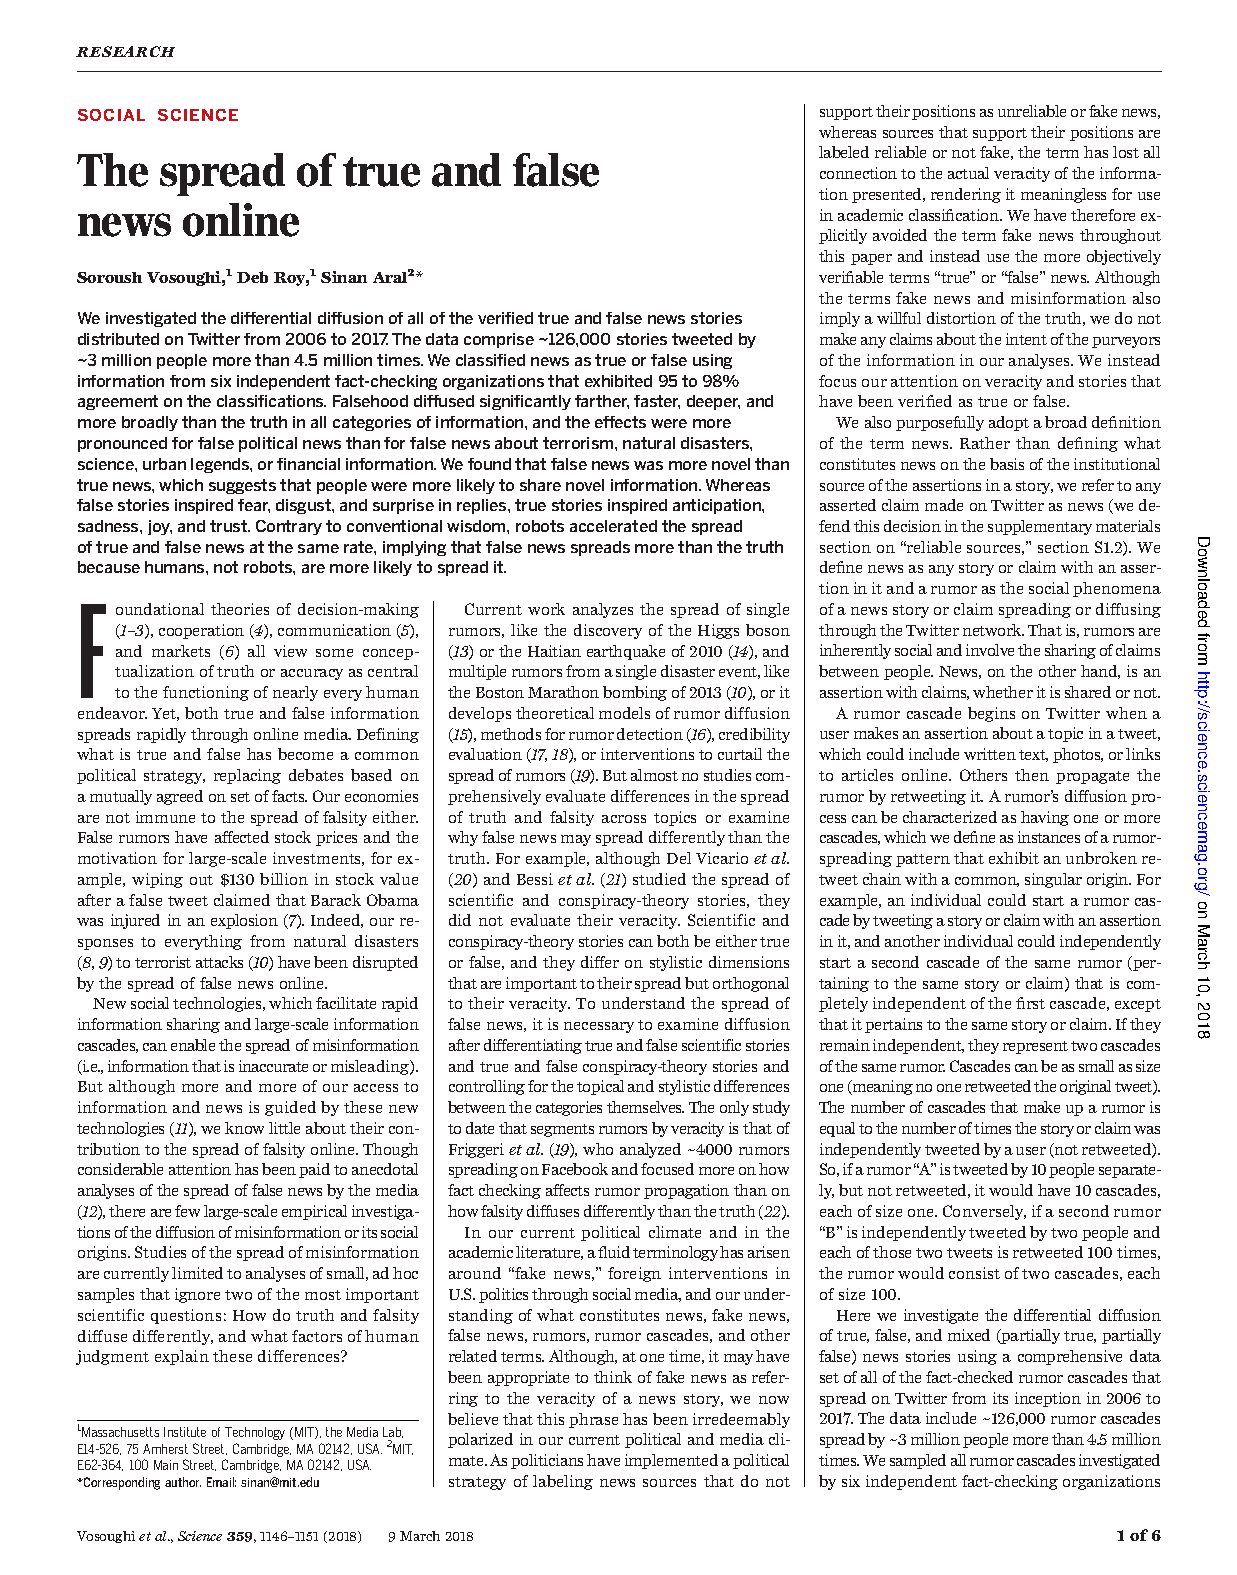
\includepdf[pages=1, scale=0.95, pagecommand=\heiti\sanhao{外\quad{}文\quad{}原\quad{}文}]{docs/translation.pdf}
\includepdf[pages=2-, scale=0.95, pagecommand={}]{docs/translation.pdf}
\end{center}

% 开题报告
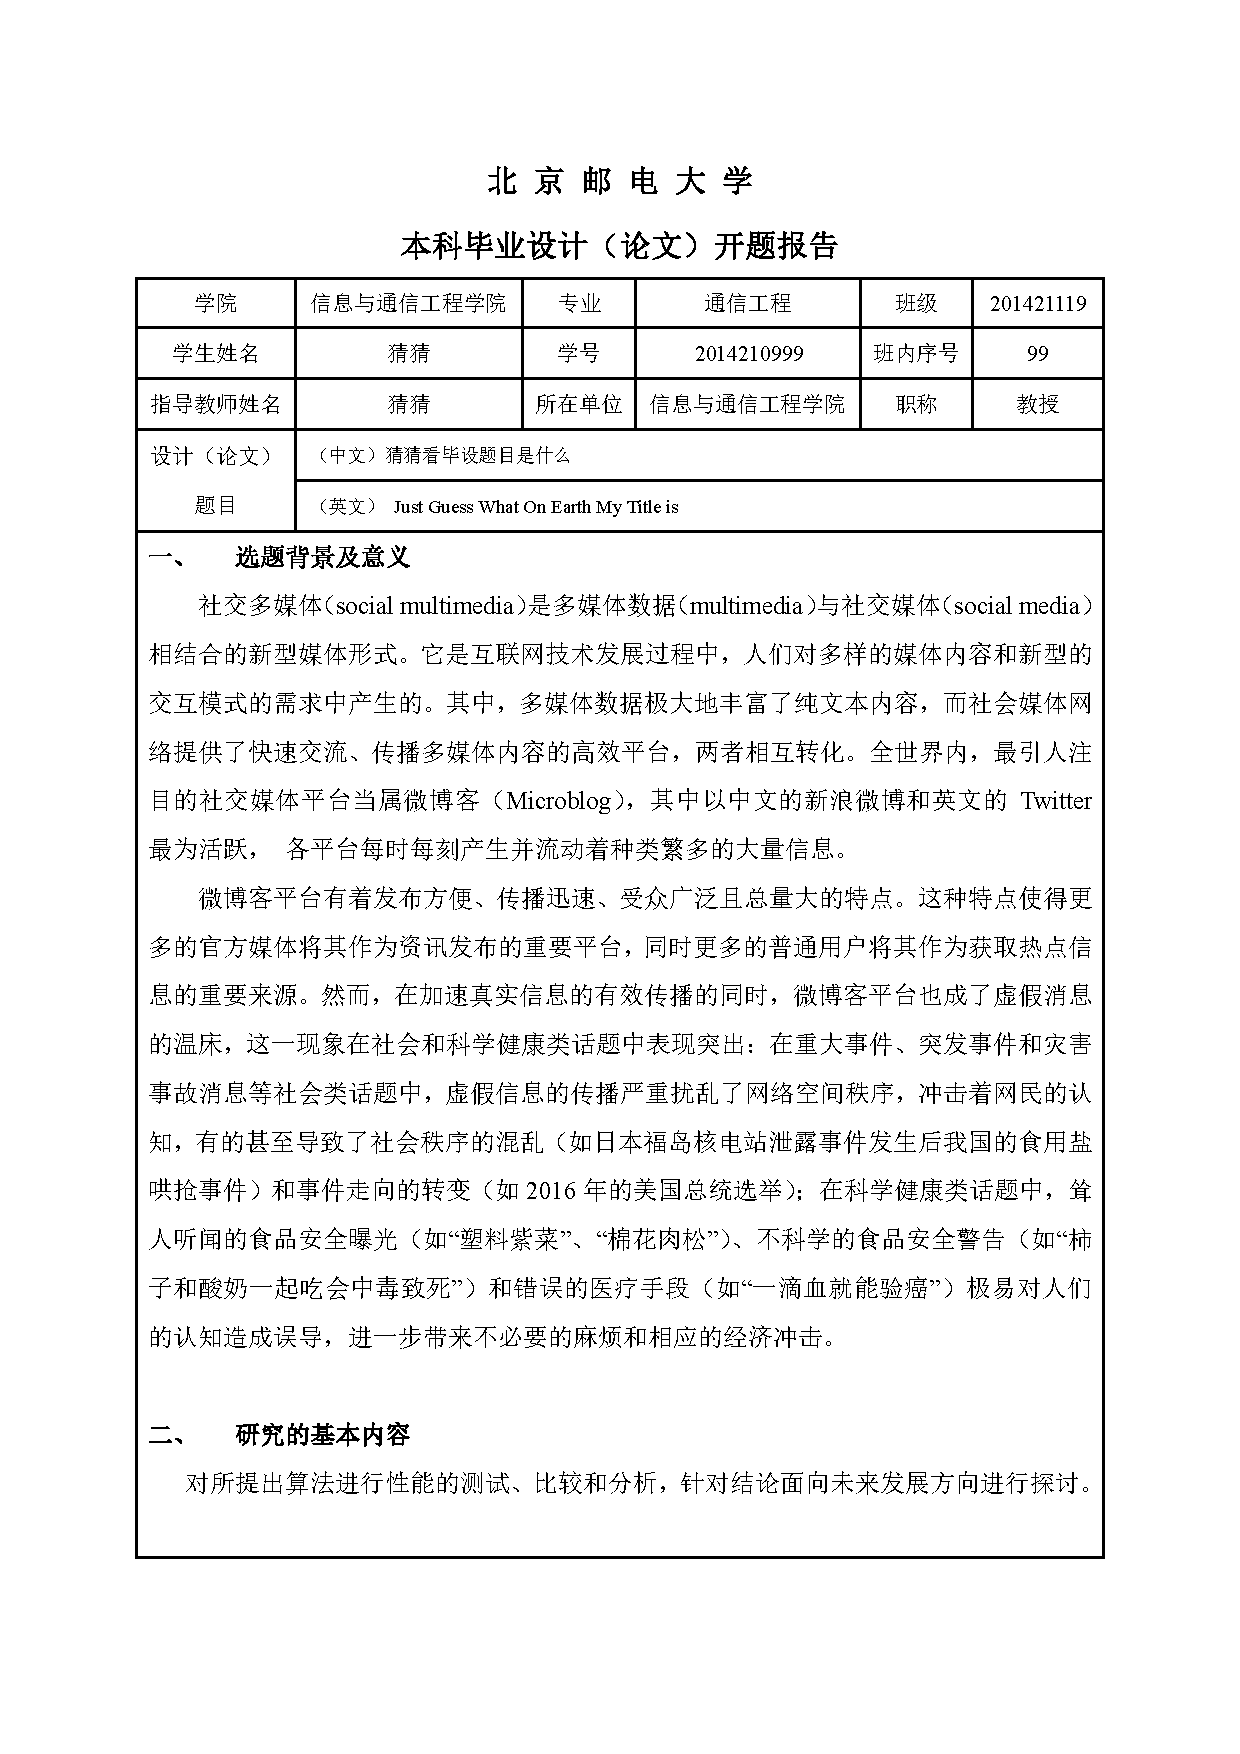
\includepdf[pages=-]{docs/openingReport.pdf} 


% 中期检查表
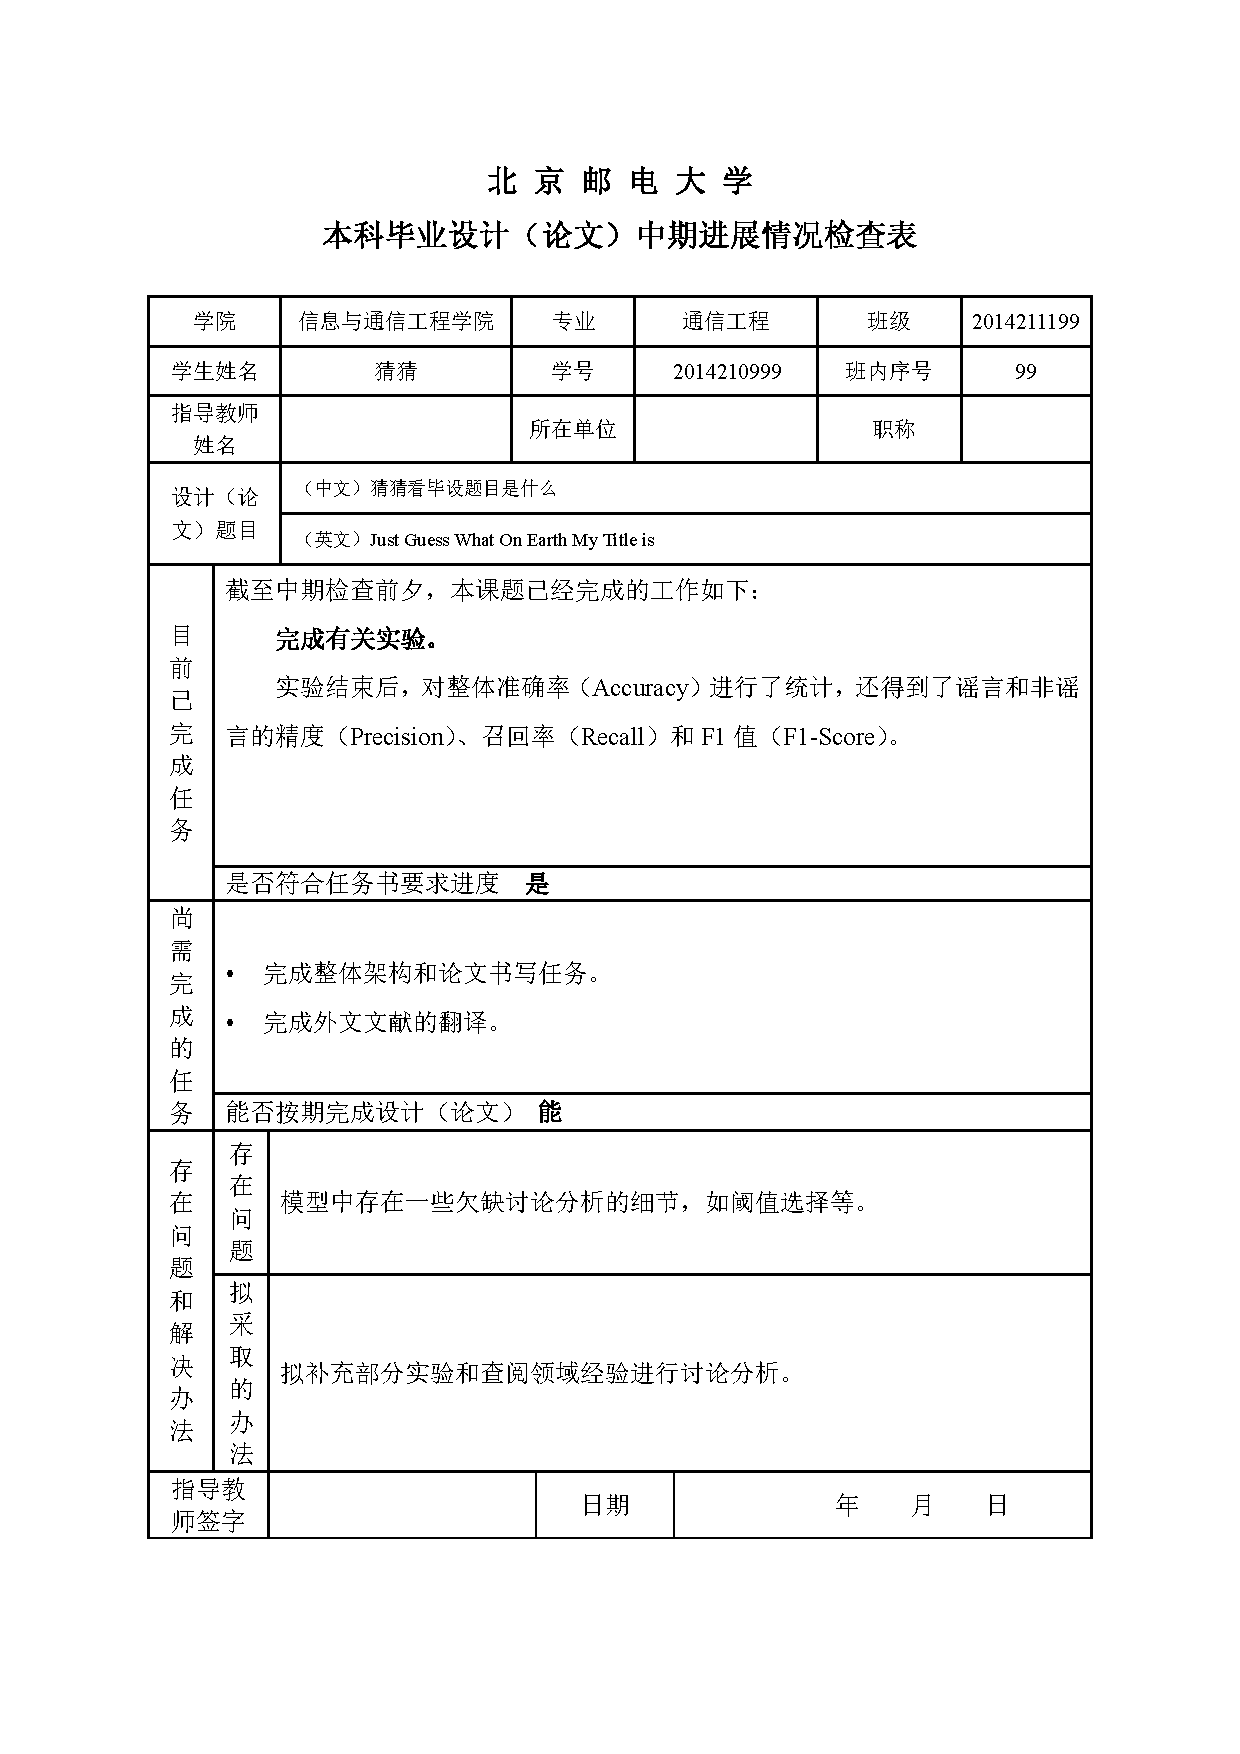
\includepdf[pages=-]{docs/interimReport.pdf} 


\end{document}